% !TeX program = xelatex
% English publication copy adapted from the handwritten transcription, pp. 1--20.
% Approved local amendment: define Omega on source p. 16, retain the domain
% in the sector integral and use {z : m+gz in Omega} after the change of variables.
\documentclass[10pt,reqno]{amsart}
\usepackage[margin=1in]{geometry}
\usepackage{amsmath,amssymb,amsthm,mathtools,bm}
\usepackage{graphicx,xcolor,enumitem,indentfirst}
\usepackage[protrusion=true,expansion=false]{microtype}
\usepackage{needspace}
\usepackage[section]{placeins}
\setcounter{tocdepth}{1}
\theoremstyle{definition}
\newtheorem{definition}{Definition}[section]
\newtheorem{lemma}[definition]{Lemma}
\newtheorem{example}[definition]{Example}
\theoremstyle{remark}
\newtheorem{remark}[definition]{Remark}
\numberwithin{equation}{section}
\numberwithin{figure}{section}
\setlength{\textfloatsep}{12pt plus 3pt minus 2pt}
\setlength{\intextsep}{10pt plus 3pt minus 2pt}
\setlength{\abovecaptionskip}{5pt}
\renewcommand{\topfraction}{.85}
\renewcommand{\bottomfraction}{.7}
\renewcommand{\textfraction}{.12}
\AddToHook{cmd/section/before}{\Needspace{6\baselineskip}}
\AddToHook{cmd/subsection/before}{\Needspace{4\baselineskip}}
% All seven diagrams below are native, editable TikZ; no image files are used.
\usepackage{tikz}
\usetikzlibrary{arrows.meta,decorations.markings,decorations.pathreplacing}
\tikzset{
  ym/base/.style={font=\small, line cap=round, line join=round},
  ym/edge/.style={draw=black, line width=.8pt},
  ym/grid/.style={draw=black!35, line width=.45pt},
  ym/path/.style={draw=black, line width=1pt},
  ym/midarrow/.style={ym/edge,
    postaction={decorate},
    decoration={markings,mark=at position .55 with
      {\arrow{Stealth[length=4.2pt,width=3.4pt]}}}},
  ym/arrow/.style={ym/edge,-{Stealth[length=4.2pt,width=3.4pt]}},
  ym/brace/.style={draw=black,line width=.55pt,
    decorate,decoration={brace,mirror,amplitude=3pt}},
  ym/dot/.style={circle,fill=black,inner sep=1.15pt}
}

\usepackage{hyperref}
\setlength{\parindent}{2em}
\setlength{\parskip}{0pt}
\linespread{1.1}
\AtBeginDocument{%
  \setlength{\abovedisplayskip}{7pt plus 2pt minus 2pt}%
  \setlength{\belowdisplayskip}{7pt plus 2pt minus 2pt}%
  \setlength{\abovedisplayshortskip}{3pt plus 1pt}%
  \setlength{\belowdisplayshortskip}{5pt plus 2pt minus 1pt}}
\raggedbottom
\clubpenalty=10000
\widowpenalty=10000
\displaywidowpenalty=10000
\allowdisplaybreaks[1]
\setlist[enumerate]{leftmargin=2em,itemsep=3pt,topsep=3pt}
\newcommand{\g}{\mathfrak g}
\newcommand{\dd}{\mathrm d}
\newcommand{\id}{\mathrm{id}}
\newcommand{\YM}{\mathrm{YM}}
\newcommand{\R}{\mathbb R}
\newcommand{\C}{\mathbb C}
\newcommand{\Z}{\mathbb Z}
\newcommand{\e}{\varepsilon}
\newcommand{\Ia}{I_{\mathrm a}}
\newcommand{\If}{I_{\mathrm f}}
\newcommand{\Uf}{\mathcal U_{\mathrm f}}
\newcommand{\Uc}{\mathcal U_{\mathrm c}}
\newcommand{\Hf}{H_{\mathrm f}}
\newcommand{\Hc}{H_{\mathrm c}}
\newcommand{\Fc}{F_{\mathrm c}}
\newcommand{\Gc}{G_{\mathrm c}}
\newcommand{\Oc}{O_{\mathrm c}}
\newcommand{\muc}{\mu_{\mathrm c}}
\DeclareMathOperator{\Ad}{Ad}
\DeclareMathOperator{\ad}{ad}
\DeclareMathOperator{\tr}{tr}
\DeclareMathOperator{\Vol}{Vol}
\setlength{\emergencystretch}{2em}
\hypersetup{pdftitle={Lattice Yang--Mills: Wilson measure and exact blocking},pdfauthor={Zexi He}}
\title[Lattice Yang--Mills: study notes]{Lattice Yang--Mills:\\Wilson measure and exact blocking}
\author{Zexi He}
\date{}
\AddToHook{cmd/@setauthors/after}{%
  \begingroup\centering\normalfont\footnotesize
  Personal study notes --- 13 November 2026\par\endgroup}
\begin{document}

\maketitle
\begin{list}{}{\leftmargin=1em\rightmargin=1em\topsep=4pt\parsep=0pt}
\item[]\small
These notes were developed from my handwritten study notes and transcribed,
translated and edited with AI assistance. They accompany the AI-generated
working exposition \cite{Exposition}, based on the OpenAI Yang--Mills Lean
project; source provenance and review limits are described in the repository
README. This installment covers the Wilson measure, exact blocking, tree gauge,
exponential coordinates and a Gaussian change of variables. It does not establish
the continuum construction. Corrections and missing references are welcome.
\end{list}

\tableofcontents
\medskip

\section{The Wilson measure}\label{sec:wilson}
We first recall the Wilson action and the lattice Yang--Mills measure.
Let $G$ be a closed subgroup of $U(N)$, with Lie algebra $\g$. Write $h_G$ for normalized Haar measure and $e_i$ for the coordinate unit vectors. Set
\begin{equation}\label{eq:display-001}
\Lambda_\ell=(\Z/\ell\Z)^4,
\qquad
\mathcal U_\ell:=G^{\Lambda_\ell\times\{1,2,3,4\}}.
\end{equation}
The positively oriented edges are $E_\ell^+=\Lambda_\ell\times\{1,2,3,4\}$.

A configuration $U\in\mathcal U_\ell$ assigns $U(x,i)\in G$ to the oriented link from $x$ to $x+e_i$;
the reverse link carries $U(x,i)^{-1}$.

The product Haar measure on $\mathcal U_\ell$ is
\begin{equation}\label{eq:display-002}
H_\ell=\bigotimes_{(x,i)\in\Lambda_\ell\times\{1,2,3,4\}}h_G.
\end{equation}

\begin{definition}[Plaquette holonomy] For $1\le i<j\le4$, define the holonomy around the plaquette in Figure~\ref{fig:plaquette} by



\begin{equation}\label{eq:plaquette-holonomy}
P_{ij}(U;x)
 =U(x,i)U(x+e_i,j)U(x+e_j,i)^{-1}U(x,j)^{-1}.
\end{equation}
\end{definition}

\begin{figure}[htbp]
\centering
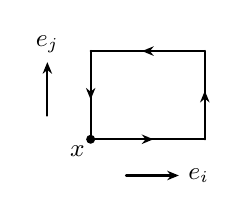
\begin{tikzpicture}[ym/base]
  \coordinate (x) at (0,0);
  \coordinate (xi) at (1.45,0);
  \coordinate (xij) at (1.45,1.12);
  \coordinate (xj) at (0,1.12);
  \draw[ym/midarrow] (x) -- (xi);
  \draw[ym/midarrow] (xi) -- (xij);
  \draw[ym/midarrow] (xij) -- (xj);
  \draw[ym/midarrow] (xj) -- (x);
  \node[ym/dot] at (x) {};
  \node[below left,inner sep=2pt] at (x) {$x$};
  \draw[ym/arrow] (.45,-.46) -- (1.12,-.46)
    node[right,inner sep=3pt] {$e_i$};
  \draw[ym/arrow] (-.55,.30) -- (-.55,.98)
    node[above,inner sep=3pt] {$e_j$};
\end{tikzpicture}
\caption{The positively oriented plaquette based at $x$.}
\label{fig:plaquette}
\end{figure}

\begin{definition}[Wilson measure]
The Wilson energy is
\begin{equation}\label{eq:wilson-energy}
W_\ell(U)=\sum_{x\in\Lambda_\ell}\sum_{i<j}
 \left(1-\frac1N\operatorname{Re}\tr P_{ij}(U;x)\right).
\end{equation}
For $\beta\in\R$, set
\begin{equation}\label{eq:partition-function}
Z_\ell(\beta):=\int_{\mathcal U_\ell}e^{-\beta W_\ell(U)}\,\dd H_\ell(U),
\end{equation}
\begin{equation}\label{eq:wilson-measure}
\dd\mu_{\ell,\beta}(U)
 =Z_\ell(\beta)^{-1}e^{-\beta W_\ell(U)}\,\dd H_\ell(U).
\end{equation}
\end{definition}

This convention makes the scaling factors explicit in subsequent renormalization-group calculations.

\begin{remark} Distances in $\Lambda_\ell$ are measured in lattice units; $\ell$ is the number of sites in each coordinate direction.
At mesh $\e$, the physical side length is $M=\e\ell$.
In four dimensions, no explicit power of $\e$ occurs in this definition of $\mu_{\ell,\beta}$.

\end{remark}

\subsection{Relation to the continuum action}
For this scaling calculation only, use the $d$-dimensional analogue $\Lambda_\ell=(\Z/\ell\Z)^d$. Consider, formally,
\begin{equation}\label{eq:display-007}
\Lambda_{M,\e}=(\e\Z/M\Z)^d,
\qquad
\mu^{\YM}(\dd A)\propto\exp\bigl(-S(A)\bigr)\,\dd A,
\end{equation}
\begin{equation}\label{eq:display-008}
S(A)=\int_{\R^d}|F_A|^2\,\dd x,
\qquad (F_A)_{ij}=[D_{A,i},D_{A,j}].
\end{equation}
Here $A$ is smooth, $D_{A,i}=\partial_i+A_i$, and the continuum curvature is the matrix coefficient of this commutator. The symbol $\dd A$ is formal; no infinite-dimensional Lebesgue measure is being defined.
The corresponding lattice expression is
\begin{equation}\label{eq:display-009}
\int_{\R^d}|F_A|^2\,\dd x
\leadsto
\e^d\sum_{x\in\Lambda_\ell}\sum_{i<j}
\operatorname{Re}\tr\bigl((F_U)_{ij}(F_U)_{ij}^*\bigr).
\end{equation}

For a lattice function $f$ with values in $\C^N$, define
\begin{equation}\label{eq:display-010}
(D_{U,i}f)(x):=\e^{-1}\bigl(U(x,i)f(x+e_i)-f(x)\bigr).
\end{equation}
Then
\begin{equation}\label{eq:display-011}
([D_{U,i},D_{U,j}]f)(x)
=(F_U)_{ij}(x)f(x+e_i+e_j).
\end{equation}
The matrix $(F_U)_{ij}(x)$ is the coefficient after extracting the common endpoint shift. The two paths are shown in Figure~\ref{fig:curvature}.

\begin{figure}[htbp]
\centering
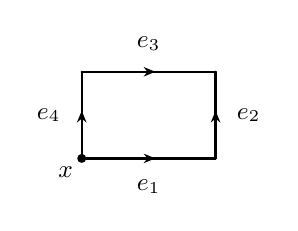
\begin{tikzpicture}[ym/base]
  \draw[ym/midarrow] (0,0) -- (1.70,0)
    node[midway,below=4pt] {$e_1$};
  \draw[ym/midarrow] (1.70,0) -- (1.70,1.10)
    node[midway,right=4pt] {$e_2$};
  \draw[ym/midarrow] (0,1.10) -- (1.70,1.10)
    node[midway,above=4pt] {$e_3$};
  \draw[ym/midarrow] (0,0) -- (0,1.10)
    node[midway,left=4pt] {$e_4$};
  \node[ym/dot] at (0,0) {};
  \node[below left,inner sep=3pt] at (0,0) {$x$};
\end{tikzpicture}
\caption{The two paths from $x$ to $x+e_i+e_j$; the top and left edges point right and up.}
\label{fig:curvature}
\end{figure}

\begin{equation}\label{eq:lattice-curvature}
(F_U)_{ij}(x)=\frac1{\e^2}\left(U_{e_1}U_{e_2}-U_{e_4}U_{e_3}\right).
\end{equation}
Thus
\begin{equation}\label{eq:display-013}
\e^d\sum_{x\in\Lambda_\ell}\sum_{i<j}
\operatorname{Re}\tr\bigl((F_U)_{ij}(F_U)_{ij}^*\bigr) =2\e^{d-4}\sum_{x\in\Lambda_\ell}\sum_{i<j}
\left(N-\operatorname{Re}\tr\bigl(P_{ij}(U;x)\bigr)\right).
\end{equation}
For $d=4$,
\begin{equation}\label{eq:display-014}
\mu_{M,\e}(\dd U)
\propto\exp\left(-C\sum_{x\in\Lambda_\ell}\sum_{i<j}
\left(N-\operatorname{Re}\tr\bigl(P_{ij}(U;x)\bigr)\right)\right) \times\dd H_{M,\e}(U).
\end{equation}
At fixed coupling, its dependence on $M,\e$ is through $\ell=M/\e$.

\begin{remark}[Normalization]
We write $C=\beta/N$. With $N$ fixed, this is a parametrization of the coupling; no large-$N$ limit is considered here.

\end{remark}

\begin{lemma}\label{lem:wilson-bound} $W_\ell$ is continuous and
\begin{equation}\label{eq:display-015}
0\le W_\ell(U)\le12\ell^4.
\end{equation}
\end{lemma}

\begin{proof}
\begin{equation}\label{eq:display-016}
W_\ell(U)=\sum_{x\in\Lambda_\ell}\sum_{i<j}
\left(1-\frac1N\operatorname{Re}\tr P_{ij}(U;x)\right).
\end{equation}
For $P\in U(N)$, each diagonal entry satisfies $|P_{aa}|\le1$.
Indeed,
\begin{equation}\label{eq:display-017}
PP^*=I\quad\Longrightarrow\quad
\sum_bP_{ab}\overline{P_{cb}}=\delta_{ac}
\quad\Longrightarrow\quad\sum_b|P_{ab}|^2=1.
\end{equation}
Hence
\begin{equation}\label{eq:display-018}
\bigl|\operatorname{Re}\tr P_{ij}(U;x)\bigr|\le N,
\end{equation}
so that
\begin{equation}\label{eq:display-019}
0\le W_\ell(U)\le\ell^4\binom42\times2=12\ell^4.
\end{equation}
\end{proof}

\subsection{Gauge invariance and observables}
For $t:\Lambda_\ell\to G$,
\begin{equation}\label{eq:display-020}
U^t(x,i)=t(x)U(x,i)t(x+e_i)^{-1}.
\end{equation}
Then
\begin{equation}\label{eq:display-021}
P_{ij}(U^t;x)=t(x)P_{ij}(U;x)t(x)^{-1},
\qquad W_\ell(U^t)=W_\ell(U).
\end{equation}
Introduce the lattice spacing $\e_n$ and physical side length $M$:
\begin{equation}\label{eq:display-022}
\e:=\e_n=\frac1n,
\qquad \ell:=\ell_{n,M}=M/\e_n.
\end{equation}
The eventual aim is to study the limits $n\to\infty$ and $M\to\infty$.

\begin{definition}[Local gauge-invariant observables]
Let $\mathcal V$ be a label set. A family of local gauge-invariant observables is written as
\begin{equation}\label{eq:display-023}
\mathcal O_{M,\e}(\nu,x;U),
\qquad\nu\in\mathcal V,\quad x\in\Lambda_\ell,\quad U\in\mathcal U_\ell.
\end{equation}

For every $\nu,x$, require that
\begin{equation}\label{eq:display-024}
U\longmapsto\mathcal O_{M,\e}(\nu,x;U)
\quad\text{is continuous, gauge invariant, and local.}
\end{equation}
Here locality means that, for every $\nu$, there is a finite set $D_\nu\subset\Z^4$ such that
$\mathcal O_{M,\e}(\nu,x;U)$ depends only on links whose endpoints lie in $x+D_\nu$, interpreted periodically.
The set $D_\nu$ is independent of $M,\e$.

Its physical support diameter is bounded by
\begin{equation}\label{eq:display-025}
\e\operatorname{diam}(D_\nu)\longrightarrow0.
\end{equation}
\end{definition}

\begin{example}[Plaquette observable] For $\nu=(i,j)$, $i<j$, take
\begin{equation}\label{eq:display-026}
\mathcal O_\ell(\nu,x;U)
 =1-\frac1N\operatorname{Re}\tr P_{ij}(U;x).
\end{equation}

\end{example}

\begin{example}[Wilson loop] Let $\gamma=(e_1,\ldots,e_q)$ be a fixed finite closed path based at $0$, where each $e_j$ denotes an oriented edge. Its translate is
\begin{equation}\label{eq:display-027}
\gamma_x=x+\gamma,
\end{equation}
\begin{equation}\label{eq:display-028}
W_\gamma(x;U)=\frac1N\tr\bigl(U_{x+e_1}\cdots U_{x+e_q}\bigr).
\end{equation}



The path itself is the label:
\begin{equation}\label{eq:display-029}
\nu:=\gamma\in\mathcal V:=\{\text{finite closed paths based at $0$}\}.
\end{equation}
\end{example}

\begin{figure}[htbp]
\centering
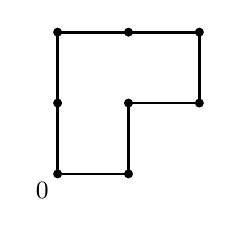
\begin{tikzpicture}[ym/base,x=.90cm,y=.90cm]
  \draw[ym/path] (0,0) -- (1,0) -- (1,1) -- (2,1)
    -- (2,2) -- (0,2) -- cycle;
  \foreach \point in {(0,0),(1,0),(1,1),(2,1),(2,2),(1,2),(0,2),(0,1)}
    \node[ym/dot] at \point {};
  \node[below left,inner sep=3pt] at (0,0) {$0$};
\end{tikzpicture}
\caption{A finite closed path based at the origin.}
\label{fig:wilson-loop}
\end{figure}

\begin{definition}[Correlation functions]
For labels $\nu_1,\ldots,\nu_k$ and sites $x_1,\ldots,x_k$, define
\begin{equation}\label{eq:display-030}
C_{M,\e,\beta}(\nu;x)
 =\int\prod_{j=1}^k\mathcal O_{M,\e}(\nu_j,x_j;U)\,\dd\mu_{\ell,\beta}(U).
\end{equation}
\end{definition}

The first objective is to study $\e\downarrow0$ at fixed $M$.
Set $\ell_{M,\e}=M/\e$ and choose $\beta:=\beta_{M,\e}$ appropriately.

\section{Exact one-step blocking}
With a suitable choice of $\beta_{M,\e}$ and suitable conditions on $\mathcal O_{M,\e}$, the objective is to study
\begin{equation}\label{eq:display-031}
C_{M,\e}(\nu;x):=C_{M,\e,\beta_{M,\e}}(\nu;x)
\end{equation}
as $\e\to0^+$. Locality and continuity alone are not a convergence theorem.

As $\e\to0^+$, the number of integration variables grows. To organize this integral, introduce a coarser configuration.

Write
\begin{equation}\label{eq:display-032}
F(U):=e^{-\beta_{M,\e}W_\ell(U)},
\qquad
O(U)=\prod_{j=1}^k\mathcal O_{M,\e}(\nu_j,x_j;U).
\end{equation}
Then
\begin{equation}\label{eq:display-033}
C_{M,\e}(\nu;x)
 =\frac{\displaystyle\int_{\Uf}O(U)F(U)\,\dd H_{M,\e}(U)}
 {\displaystyle\int_{\Uf}F(U)\,\dd H_{M,\e}(U)}.
\end{equation}
Write $\Uf:=\mathcal U_\ell$ and $\Hf:=H_{M,\e}=H_\ell$; the subscript $\mathrm f$ denotes the fine lattice.

Let $V$ be a coarse configuration with product Haar measure $\dd\Hc(V)$:
\begin{equation}\label{eq:display-034}
V\in\Uc:=G^{E^+_{\ell/L}},\qquad L>1.
\end{equation}
Here $L$ is an integer dividing $\ell$.

Insert the normalization
\begin{equation}\label{eq:blocking-normalization}
1=\int_{\Uc}K(U,V)\,\dd\Hc(V),\qquad\forall U.
\end{equation}
A nonnegative measurable function $K(U,V)$ satisfying~\eqref{eq:blocking-normalization} is called a blocking kernel density.

Thus
\begin{equation}\label{eq:display-036}
\begin{aligned}
\int_{\Uf}O(U)F(U)\,\dd\Hf(U)
&=\int_{\Uf\times\Uc}O(U)F(U)K(U,V)\,\dd\Hc(V)\,\dd\Hf(U)\\
&=\int_{\Uc}\left(\int_{\Uf}O(U)F(U)K(U,V)\,\dd\Hf(U)\right)\dd\Hc(V).
\end{aligned}
\end{equation}
Denote the inner integral by $\Gc(V)$.

Similarly, set
\begin{equation}\label{eq:coarse-density}
\Fc(V):=\int_{\Uf}F(U)K(U,V)\,\dd\Hf(U).
\end{equation}
This gives the \textbf{exact one-step blocking identity}:
\begin{equation}\label{eq:display-038}
C_{M,\e}(\nu;x)
 =\frac{\displaystyle\int_{\Uc}\Gc(V)\,\dd\Hc(V)}
 {\displaystyle\int_{\Uc}\Fc(V)\,\dd\Hc(V)}.
\end{equation}
\begin{equation}\label{eq:display-039}
\text{coarse probability measure:}\qquad
\dd\muc(V)=\frac{\Fc(V)}{Z}\,\dd\Hc(V).
\end{equation}
Here $Z=Z_\ell(\beta_{M,\e})=\int\Fc\,\dd\Hc$, and $\Fc$ is the effective density.

For $\Fc(V)>0$, define
\begin{equation}\label{eq:coarse-observable}
\Oc(V)
:=\frac{\Gc(V)}{\Fc(V)} =\frac{\displaystyle\int_{\Uf}K(U,V)O(U)F(U)\,\dd\Hf(U)}
 {\displaystyle\int_{\Uf}K(U,V)F(U)\,\dd\Hf(U)}.
\end{equation}
Therefore
\begin{equation}\label{eq:display-041}
C_{M,\e}(\nu;x)=\int_{\Uc}\Oc(V)\,\dd\muc(V).
\end{equation}

\section{A two-dimensional example}

For this example, consider a single square coarse plaquette $P$ of mesh $\e$ in two dimensions.
Subdivide $P$ into $L^2$ fine plaquettes, as illustrated schematically in Figure~\ref{fig:fine-coarse}. The fine mesh is
\begin{equation}\label{eq:display-042}
\delta=\e/L.
\end{equation}

\begin{figure}[htbp]
\centering
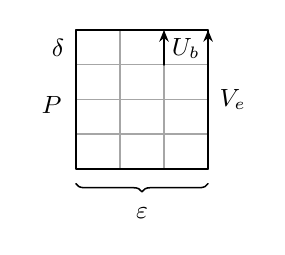
\begin{tikzpicture}[ym/base,x=.56cm,y=.44cm]
  \foreach \x in {0,1,2,3}
    \draw[ym/grid] (\x,0) -- (\x,4);
  \foreach \y in {0,1,2,3,4}
    \draw[ym/grid] (0,\y) -- (3,\y);
  \draw[ym/edge] (0,0) rectangle (3,4);
  \draw[ym/arrow] (2,3) -- (2,4);
  \node[anchor=west,inner sep=2pt] at (2.04,3.48) {$U_b$};
  \draw[ym/arrow] (3,0) -- (3,4);
  \node[anchor=west,inner sep=4pt] at (3,2) {$V_e$};
  \node[anchor=east,inner sep=4pt] at (0,3.50) {$\delta$};
  \node[anchor=east,inner sep=5pt] at (0,1.85) {$P$};
  \draw[ym/brace] (0,-.43) -- (3,-.43)
    node[midway,below=5pt] {$\varepsilon$};
\end{tikzpicture}
\caption{Fine links and a coarse boundary link of a plaquette $P$ (schematic).}
\label{fig:fine-coarse}
\end{figure}

On the fine edges in $P$, put the Wilson measure
\begin{equation}\label{eq:display-043}
\mu_\delta(\dd U)=\frac1{Z_\delta}\prod_{q\in\mathcal P}Q_\delta(U_q)
\prod_{b\in E_\delta^+}\dd U_b,
\qquad
Q_\delta(U)\propto\exp\left(-\beta\left(1-\frac1N\operatorname{Re}\tr U\right)\right).
\end{equation}
Define
\begin{equation}\label{eq:display-044}
V_e=U_{b_1}\cdots U_{b_L},
\qquad\Pi_L:U\longmapsto V.
\end{equation}
We compute the pushforward $(\Pi_L)_*\mu_\delta$. In this example $\Gc$ is a bounded test function, $\mathcal P$ is the set of fine plaquettes in $P$, and $\partial E_\delta^+$ consists of the fine boundary edges.
\begin{equation}\label{eq:display-045}
\begin{aligned}
\int\Gc(V)\,(\Pi_L)_*\mu_\delta(\dd V)
&=\int\Gc(\Pi_LU)\,\mu_\delta(\dd U)\\
&\propto\int\Gc(\Pi_LU)\prod_{q\in\mathcal P}Q_\delta(U_q)
 \prod_{b\in E_\delta^+}\dd U_b\\
&\propto\int\Gc(\Pi_LU)
 \left(\int_{G^{E_\delta^+\setminus\partial E_\delta^+}}
 \prod_{q\in\mathcal P}Q_\delta(U_q)
 \prod_{b\in E_\delta^+\setminus\partial E_\delta^+}\dd U_b\right)
 \prod_{b\in\partial E_\delta^+}\dd U_b.
\end{aligned}
\end{equation}

The elementary merging identity is illustrated in Figure~\ref{fig:merging}.
\begin{figure}[htbp]
\centering
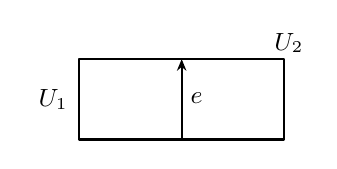
\begin{tikzpicture}[ym/base]
  \draw[ym/edge] (0,0) rectangle (2.60,1.02);
  \draw[ym/arrow] (1.30,0) -- (1.30,1.02);
  \node[anchor=west,inner sep=3pt] at (1.30,.53) {$e$};
  \node[anchor=east,inner sep=4pt] at (0,.51) {$U_1$};
  \node[anchor=south west,inner sep=2pt] at (2.40,1.02) {$U_2$};
\end{tikzpicture}
\caption{Two adjacent plaquettes sharing the link $e$.}
\label{fig:merging}
\end{figure}

\begin{equation}\label{eq:display-046}
\int_GQ_\delta(U_1U_e^{-1})Q_\delta(U_eU_2)\,\dd U_e =(Q_\delta*Q_\delta)(U_1U_2).
\end{equation}
Only the outer boundary holonomy remains. Here $(f*g)(W):=\int_G f(WV^{-1})g(V)\,\dd h_G(V)$ denotes convolution.

Consequently,
\begin{equation}\label{eq:display-047}
\int_{G^{E_\delta^+\setminus\partial E_\delta^+}}
\prod_{q\in\mathcal P}Q_\delta(U_q)
\prod_{b\in E_\delta^+\setminus\partial E_\delta^+}\dd U_b
=K_{\delta,P}\bigl(U(\partial P)\bigr).
\end{equation}
The function $K_{\delta,P}$ depends only on the boundary holonomy of $P$.

Therefore
\begin{equation}\label{eq:display-048}
\begin{aligned}
\int\Gc(V)\,(\Pi_L)_*\mu_\delta(\dd V)
&\propto\int\Gc(\Pi_LU)K_{\delta,P}\bigl(U(\partial P)\bigr)
\prod_{b\in\partial E_\delta^+}\dd U_b\\
&=\int\Gc(V)K_{\delta,P}\bigl(V(\partial P)\bigr)
(\Pi_L)_*\left(\prod_{b\in\partial E_\delta^+}\dd U_b\right)(\dd V).
\end{aligned}
\end{equation}
Here
\begin{equation}\label{eq:display-049}
(\Pi_L)_*\left(\prod_{b\in\partial E_\delta^+}\dd U_b\right)(\dd V)
=\prod_{e\in E_\e^+}\dd V_e.
\end{equation}
This is deterministic blocking, described by the probability kernel
\begin{equation}\label{eq:display-050}
K(U,\dd V)=\delta_{\Pi_L(U)}(\dd V).
\end{equation}

\section{A smooth blocking kernel}
Return to four dimensions. We now choose a blocking density so that $V$ records local information about $U$.

The construction follows \cite[Section~11, (11.1)--(11.2)]{Exposition}.\par\smallskip

\subsection{Coarse-link holonomy}

The coarse link from $x$ to $x+e_i$ corresponds to a fine path from $Lx$ to $Lx+Le_i$; see Figure~\ref{fig:coarse-link}.

\begin{figure}[htbp]
\centering
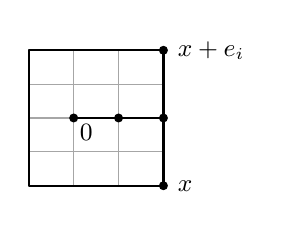
\begin{tikzpicture}[ym/base,x=.57cm,y=.43cm]
  \foreach \x in {0,1,2,3}
    \draw[ym/grid] (\x,0) -- (\x,4);
  \foreach \y in {0,1,2,3,4}
    \draw[ym/grid] (0,\y) -- (3,\y);
  \draw[ym/edge] (0,0) rectangle (3,4);
  \draw[ym/path] (1,2) -- (3,2);
  \draw[ym/path] (3,0) -- (3,4);
  \foreach \point in {(1,2),(2,2),(3,2),(3,0),(3,4)}
    \node[ym/dot] at \point {};
  \node[below right,inner sep=2pt] at (1,2) {$0$};
  \node[anchor=west,inner sep=5pt] at (3,0) {$x$};
  \node[anchor=west,inner sep=5pt] at (3,4) {$x+e_i$};
\end{tikzpicture}
\caption{A coarse link and its fine-lattice realization (schematic).}
\label{fig:coarse-link}
\end{figure}

\begin{equation}\label{eq:display-051}
Q(U)_i(x):=U_i(Lx)U_i(Lx+e_i)\cdots U_i\bigl(Lx+(L-1)e_i\bigr).
\end{equation}
Allow $V$ to fluctuate around $Q(U)$.

The mismatch is
\begin{equation}\label{eq:display-052}
V_eQ(U)_e^{-1}\qquad\text{(mismatch)}.
\end{equation}
For $W\in G$, set
\begin{equation}\label{eq:display-053}
q_G(W):=1-\frac1N\operatorname{Re}\tr W =\frac1{2N}\|W-I\|_{\mathrm{HS}}^2\ge0.
\end{equation}
Assign to this mismatch the weight
\begin{equation}\label{eq:display-054}
\exp\left(-a\beta\,q_G\bigl(V_eQ(U)_e^{-1}\bigr)\right).
\end{equation}
Here $a>0$ is fixed and $\beta:=\beta_{M,\e}>0$.
The weight is maximal when $V_e=Q(U)_e$. The Hilbert--Schmidt norm is $\|B\|_{\mathrm{HS}}^2=\tr(BB^*)$.

Define
\begin{equation}\label{eq:display-055}
z_n(\beta):=\int_Ge^{-a\beta q_G(W)}\,\dd h_G(W)\in[e^{-a\beta},1].
\end{equation}

\begin{equation}\label{eq:smooth-kernel}
K_\beta(U,V):=\prod_{e\in E_{\ell/L}^+}
\frac{e^{-a\beta q_G(V_eQ(U)_e^{-1})}}{z_n(\beta)}.
\end{equation}
Right invariance of Haar measure gives
\begin{equation}\label{eq:display-057}
\int_Ge^{-a\beta q_G(V_eQ(U)_e^{-1})}\,\dd V_e
=\int_Ge^{-a\beta q_G(W)}\,\dd W =z_n(\beta).
\end{equation}
Thus
\begin{equation}\label{eq:display-058}
\int_{\Uc}K_\beta(U,V)\,\dd\Hc(V)=1.
\end{equation}
\begin{remark} At fixed $\beta>0$, as $a\to\infty$,
\begin{equation}\label{eq:display-059}
K_{\beta,a}(U,V)\,\dd\Hc(V)\Longrightarrow\delta_{Q(U)}(\dd V).
\end{equation}
\end{remark}

The coarse density is therefore
\begin{equation}\label{eq:display-060}
\begin{aligned}
\Fc(V)
&=\int_{\mathcal U_\ell}K_\beta(U,V)e^{-\beta W_\ell(U)}\,\dd\Hf(U)\\
&=z_n(\beta)^{-\#E_{\ell/L}^+}\int_{\Uf}
\exp\left\{-\beta\left[W_\ell(U)
+a\sum_{e\in E_{\ell/L}^+}q_G\bigl(V_eQ(U)_e^{-1}\bigr)\right]\right\}
\dd\Hf(U).
\end{aligned}
\end{equation}
\section{Tree gauge}
We follow \cite[Section~11, Lemma~11.2]{Exposition}.

Set
\begin{equation}\label{eq:blocking-action}
A(V,U):=W_\ell(U)+a\sum_{e\in E_{\ell/L}^+}q_G\bigl(V_eQ(U)_e^{-1}\bigr).
\end{equation}
The path products transform according to
\begin{equation}\label{eq:display-062}
Q(U^g)_i(x)=g(Lx)Q(U)_i(x)g(Lx+Le_i)^{-1}.
\end{equation}

If $g(Lx)=1$ at every embedded coarse site, then
\begin{equation}\label{eq:display-063}
Q(U^g)=Q(U)
\quad\Longrightarrow\quad
A(V,U^g)=A(V,U).
\end{equation}
We now integrate out the gauge freedom in
\begin{equation}\label{eq:display-064}
\int_{\Uf}\exp\bigl(-A(V,U)\bigr)\,\dd\Hf(U)
\end{equation}
by fixing the links of a rooted tree in each block.

\begin{figure}[htbp]
\centering
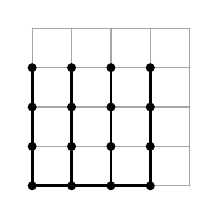
\begin{tikzpicture}[ym/base,x=.50cm,y=.50cm]
  \foreach \x in {0,1,2,3,4}
    \draw[ym/grid] (\x,0) -- (\x,4);
  \foreach \y in {0,1,2,3,4}
    \draw[ym/grid] (0,\y) -- (4,\y);
  \draw[ym/path] (0,0) -- (3,0);
  \foreach \x in {0,1,2,3}
    \draw[ym/path] (\x,0) -- (\x,3);
  \foreach \x in {0,1,2,3}
    \foreach \y in {0,1,2,3}
      \node[ym/dot] at (\x,\y) {};
\end{tikzpicture}
\caption{A rooted block tree, shown in two dimensions; dark edges form the tree.}
\label{fig:block-tree}
\end{figure}

In each coarse block $Lx+\{0,\ldots,L-1\}^4$, choose a tree such that
\begin{enumerate}[label=(\roman*)]
\item its vertices are exactly $Lx+\{0,\ldots,L-1\}^4$;
\item its root is $Lx$.
\end{enumerate}
Any such tree suffices for this identity; Figure~\ref{fig:block-tree} shows a two-dimensional example.
Let $T$ denote the union of their edges, represented with the positive lattice orientation.

\begin{definition}[Tree gauge] $U$ is in tree gauge if $U|_T=\id$.

\end{definition}

\begin{lemma}\label{lem:tree-gauge} Every configuration can be transformed into tree gauge by a gauge transformation.\end{lemma}

\begin{proof} Consider $U\in\Uf$. Set $g=\id$ at each root.
Suppose $g(x)$ has been determined at a parent $x$. Write $U_{xy}$ for the link from $x$ to its child $y$, using the inverse if this reverses the positive lattice orientation. Define
\begin{equation}\label{eq:display-065}
g(y):=g(x)U_{xy},\qquad\forall y\text{ such that }y\text{ has parent }x.
\end{equation}
Then
\begin{equation}\label{eq:display-066}
U_{xy}^g
=g(x)U_{xy}g(y)^{-1} =g(x)U_{xy}\bigl(g(x)U_{xy}\bigr)^{-1} =\id.
\end{equation}
\end{proof}

Write
\begin{equation}\label{eq:remaining-links}
I:=E_\ell^+\setminus T.
\end{equation}
Writing $e_-,e_+$ for the initial and terminal vertices of $e$, the remaining configuration is determined by
\begin{equation}\label{eq:display-068}
u_e:=g(e_-)U_eg(e_+)^{-1},\qquad e\in I
\end{equation}

For $u\in G^I$, define
\begin{equation}\label{eq:display-069}
U_T(u)_e=
\begin{cases}
1,&e\in T,\\
u_e,&e\in I.
\end{cases}
\end{equation}
To integrate out the links in $T$, write
\begin{equation}\label{eq:display-070}
J(U):=\exp\bigl(-A(V,U)\bigr).
\end{equation}
Then
\begin{equation}\label{eq:display-071}
\begin{aligned}
\int_{\Uf}J(U)\,\dd\Hf(U)
&=\int_{\Uf}J\bigl(U_T(u)\bigr)\,\dd\Hf(U)
\qquad\text{by gauge invariance}\\
&=\int_{G^T}\left(\int_{G^I}J\bigl(U_T(u)\bigr)
\prod_{e\in I}\dd U_e\right)\prod_{e\in T}\dd U_e.
\end{aligned}
\end{equation}
For each fixed collection of tree links, $g$ depends only on those links. Under the change of variables
\begin{equation}\label{eq:display-072}
U_e\longmapsto u_e=g(e_-)U_eg(e_+)^{-1}
\end{equation}
left and right Haar invariance give $\dd U_e=\dd u_e$ for $e\in I$. The normalized integral over $G^T$ is one, so the expression equals
\begin{equation}\label{eq:display-073}
\int_{G^I}J\bigl(U_T(u)\bigr)\prod_{e\in I}\dd u_e.
\end{equation}
Write $\dd h_G^I(u)=\prod_{e\in I}\dd u_e$.

Consequently,
\begin{equation}\label{eq:display-074}
\int_{\Uf}J(U)\,\dd\Hf(U)
=\int_{G^I}J\bigl(U_T(u)\bigr)\prod_{e\in I}\dd u_e.
\end{equation}

It follows that
\begin{equation}\label{eq:display-075}
\boxed{
\Fc(V)=z_n(\beta)^{-\#E_{\ell/L}^+}
\int_{G^I}e^{-\beta A(V,U_T(u))}\,\dd h_G^I(u).
}
\end{equation}
\section{Exponential coordinates and sectors}
We express the remaining group-valued links in local exponential coordinates.

Near the identity, write $U=e^X$. Equip $\g$ with the inner product $\langle X,Y\rangle_\g=\operatorname{Re}\tr(X^*Y)$ and $G$ with the induced left-invariant Riemannian metric. Then
\begin{equation}\label{eq:display-076}
\boxed{
\dd h_G(e^X)=\zeta_Gj_G(X)\,\dd X,\qquad |X|_{\g}<r_G.
}
\end{equation}
Here
\begin{equation}\label{eq:display-077}
\zeta_G=\frac1{\Vol(G)},
\end{equation}
$r_G>0$ is such that $X\mapsto e^X$ is a diffeomorphism onto its image for $|X|_\g<r_G$,
\begin{equation}\label{eq:display-078}
j_G(X)=\left|\det_{\g}\left(\int_0^1e^{-t\ad X}\,\dd t\right)\right|,
\qquad(\ad X)Y:=[X,Y].
\end{equation}
\begin{remark} $j_G>0$ and is smooth on $|X|_\g<r_G$.
\begin{equation}\label{eq:display-079}
j_G(0)=1.
\end{equation}
\end{remark}

\begin{remark} For $G=U(1)$, $j_G(X)\equiv1$.\end{remark}

The volume formula is derived in Appendix~\ref{sec:haar-appendix}.

Choose a smooth $\chi:G\to[0,1]$ supported inside the image of $\{X:|X|_\g<r_G\}$. Then
\begin{equation}\label{eq:display-080}
\int_G\chi(U)f(U)\,\dd h_G(U)
=\zeta_G\int_{|X|_\g<r_G}\chi(e^X)f(e^X)j_G(X)\,\dd X.
\end{equation}
The full integral splits exactly as
\begin{equation}\label{eq:display-081}
\int_Gf\,\dd h_G
=\int_G\chi f\,\dd h_G+\int_G(1-\chi)f\,\dd h_G.
\end{equation}

\begin{remark} To describe fluctuations around a fixed reference link $R\in G$, write
\begin{equation}\label{eq:display-082}
U=e^XR.
\end{equation}
Right invariance gives
\begin{equation}\label{eq:display-083}
\dd h_G(e^XR)=\zeta_Gj_G(X)\,\dd X.
\end{equation}
\end{remark}

For the fluctuation-integral organization, compare \cite[Section~2, pp.~265--268]{Bal87}.

Apply this to the integral
\begin{equation}\label{eq:display-084}
\int_{G^I}e^{-\beta A(V,U_T(u))}\,\dd h_G^I(u).
\end{equation}
The cutoff decomposition is an exact identity.

Fix $V$ and choose a reference link for each $e\in I$:
\begin{equation}\label{eq:display-085}
R_e(V)\in G.
\end{equation}
Split each link factor as
\begin{equation}\label{eq:display-086}
1=\chi\bigl(U_eR_e(V)^{-1}\bigr)
+\left[1-\chi\bigl(U_eR_e(V)^{-1}\bigr)\right].
\end{equation}
On the support of the first term, $U_e$ has the unique representation
\begin{equation}\label{eq:display-087}
\exists y_e\in\{X\in\g:|X|_\g<r_G\}\quad\text{s.t.}\quad U_e=e^{y_e}R_e(V).
\end{equation}
Multiplying over $e\in I$ gives
\begin{equation}\label{eq:display-088}
\begin{aligned}
1&=\prod_{e\in I}\left(\chi\bigl(U_eR_e(V)^{-1}\bigr)
+\left[1-\chi\bigl(U_eR_e(V)^{-1}\bigr)\right]\right)\\
&=\sum_{\Ia\subset I}
\prod_{e\in\Ia}\chi\bigl(U_eR_e(V)^{-1}\bigr)
\prod_{e\in\If=I\setminus\Ia}\left[1-\chi\bigl(U_eR_e(V)^{-1}\bigr)\right].
\end{aligned}
\end{equation}
The links in $\Ia$ are called active, and those in $\If=I\setminus\Ia$ are called frozen.

Each term is called a sector. Fix $\Ia,\If$ and write
\begin{equation}\label{eq:display-089}
U_e=
\begin{cases}
e^{y_e}R_e(V),&\text{for some }y_e\in\{X\in\g:|X|_\g<r_G\},\quad e\in\Ia,\\
Y_e,&e\in\If.
\end{cases}
\end{equation}
The full configuration is
\begin{equation}\label{eq:display-090}
U(V,Y,y)_e=
\begin{cases}
1,&e\in T,\\
e^{y_e}R_e(V),&e\in\Ia,\\
Y_e,&e\in\If.
\end{cases}
\end{equation}
For the active links, the change of variables gives
\begin{equation}\label{eq:display-091}
\dd h_G(U_e)=\zeta_Gj_G(y_e)\,\dd y_e,\qquad e\in\Ia.
\end{equation}
Therefore
\begin{equation}\label{eq:display-092}
\dd h_G(u)=\zeta_G^{|\Ia|}
\left(\prod_{e\in\Ia}j_G(y_e)\right)\dd y\,\dd h_G^{\If}(Y),
\qquad\dd y=\prod_{e\in\Ia}\dd y_e.
\end{equation}
Substituting $U(V,Y,y)$ into the action, set
\begin{equation}\label{eq:sector-action}
\varphi(V,Y,y):=A\bigl(V,U(V,Y,y)\bigr),
\end{equation}
\begin{equation}\label{eq:sector-cutoff}
\Theta(V,Y,y):=
\prod_{e\in\Ia}\chi(e^{y_e})
\prod_{e\in\If}\left[1-\chi\bigl(Y_eR_e(V)^{-1}\bigr)\right].
\end{equation}
Write
\begin{equation}\label{eq:display-095}
\prod_{e\in\Ia}j_G(y_e)
=\exp\left(\sum_{e\in\Ia}\log j_G(y_e)\right).
\end{equation}

Write
\begin{equation}\label{eq:haar-correction}
\psi(V,Y,y):=-\sum_{e\in\Ia}\log j_G(y_e)
\qquad\text{(Haar correction)}.
\end{equation}
% User-approved local amendment: make the chart domain explicit.
Choose an orthonormal basis of $\g$ and identify the active coordinates with $\R^d$, where $d:=|\Ia|\dim_{\R}\g$. The chart domain is
\begin{equation}\label{eq:chart-domain}
\boxed{
\Omega:=\left\{y\in\g^{\Ia}:|y_e|_{\g}<r_G
\text{ for every }e\in\Ia\right\}\subset\R^d.
}
\end{equation}
The contribution of this sector to the tree-gauge integral is
\begin{equation}\label{eq:display-098}
\zeta_G^{|\Ia|}\int_{G^{\If}}\dd h_G^{\If}(Y)
\int_{\Omega}\Theta(V,Y,y)e^{-(\beta\varphi+\psi)(V,Y,y)}\,\dd y.
\end{equation}
\section{Rewriting the integral as a Gaussian expectation}
Fix the coarse configuration $V$ and the frozen variables $Y$, and suppress them in the notation.

The active-coordinate integral is
\begin{equation}\label{eq:display-099}
\int_{\Omega}\Theta(y)e^{-(\beta\varphi+\psi)(y)}\,\dd y.
\end{equation}
To extract a Gaussian part, use the following identity.

\begin{lemma}[Gaussian change of variables]\label{lem:gaussian-change}
Let $B\in L^1(\R^d)$, $g>0$, $m\in\R^d$, and let $C$ be a symmetric positive-definite matrix. Then
\begin{equation}\label{eq:gaussian-identity}
\int_{\R^d}B(y)\,\dd y
=(2\pi g^2)^{d/2}(\det C)^{1/2} \times\int_{\R^d}
 e^{\frac12z^{\mathsf T}C^{-1}z}B(m+gz)\,\dd\mu_C(z),
\end{equation}

Here $\mu_C=\mathcal N(0,C)$.

\end{lemma}

Taking $g:=\beta^{-1/2}$ gives
\begin{equation}\label{eq:display-101}
\begin{aligned}
&\int_{\Omega}\Theta(y)e^{-(\beta\varphi+\psi)(y)}\,\dd y\\
&=\int_{\{z\in\R^d:\,m+gz\in\Omega\}}\Theta(m+gz)\\
&\qquad\times\exp\left\{-g^{-2}\varphi(m+gz)-\psi(m+gz)
+\frac12z^{\mathsf T}C^{-1}z\right\}\,\dd\mu_C(z)
\times(2\pi g^2)^{d/2}(\det C)^{1/2}.
\end{aligned}
\end{equation}
The intended choice of $m$ removes the linear term, while $C$ matches the quadratic term.

The next step would be to find $m$ satisfying $\nabla_y\varphi(m)=0$ and establish positive definiteness of the Hessian. These tasks are beyond the present installment.

\appendix
\section{Haar measure in exponential coordinates}\label{sec:haar-appendix}
\begin{lemma}[Haar density]\label{lem:haar-density}
Let $G$ be a compact, connected matrix Lie group, equipped with the metric specified above. Then
\begin{equation}\label{eq:display-102}
\boxed{
\dd h_G(e^X)=\zeta_Gj_G(X)\,\dd X,\qquad |X|_{\g}<r_G.
}
\end{equation}
Here
\begin{equation}\label{eq:display-103}
\zeta_G=\frac1{\Vol(G)},
\end{equation}
$r_G>0$ is such that $X\mapsto e^X$ is a diffeomorphism onto its image for $|X|_\g<r_G$, and
\begin{equation}\label{eq:display-104}
j_G(X)=\left|\det_{\g}\left(\int_0^1e^{-t\ad X}\,\dd t\right)\right|,
\qquad (\ad X)Y:=[X,Y].
\end{equation}
\end{lemma}

\begin{remark} $j_G>0$ and is smooth on $|X|_\g<r_G$, and $j_G(0)=1$.\end{remark}

\begin{remark} For $G=U(1)$, $j_G(X)\equiv1$.\end{remark}

\begin{proof} In this appendix $d=\dim_\R\g$. Let $\dd\operatorname{vol}_G(U)$ be the Riemannian volume measure induced by
$\langle\cdot,\cdot\rangle_\g$. We have
\begin{equation}\label{eq:display-105}
\dd h_G=\zeta_G\,\dd\operatorname{vol}_G.
\end{equation}
\smallskip\noindent\emph{Step 1: the coordinate volume formula.}
For a coordinate parametrization $\Phi:\mathcal O\subset\R^d\to G$, define
\begin{equation}\label{eq:display-106}
g_{ab}(x):=
\left\langle\frac{\partial\Phi}{\partial x^a}(x),
\frac{\partial\Phi}{\partial x^b}(x)\right\rangle_{T_{\Phi(x)}G}
\qquad\text{(Gram matrix)}.
\end{equation}
Then
\begin{equation}\label{eq:display-107}
\dd\operatorname{vol}_G\bigl(\Phi(x)\bigr)
=\sqrt{\det\bigl(g_{ab}(x)\bigr)}\,\dd x^1\cdots\dd x^d.
\end{equation}
\smallskip\noindent\emph{Step 2: exponential coordinates.}

Choose an orthonormal basis $E_1,\ldots,E_d$ of $\g$ and write
\begin{equation}\label{eq:display-108}
X=\sum_{a=1}^d x^aE_a,
\qquad \dd X=\dd x^1\cdots\dd x^d.
\end{equation}

For $\Phi(X)=e^X$,
\begin{equation}\label{eq:display-109}
\frac{\partial e^X}{\partial x^a}=D\exp_X[E_a].
\end{equation}
Therefore
\begin{equation}\label{eq:display-110}
\begin{aligned}
g_{ab}(x)
&=\bigl\langle D\exp_X[E_a],D\exp_X[E_b]\bigr\rangle_{T_{e^X}G}\\
&=\bigl\langle e^{-X}D\exp_X[E_a],e^{-X}D\exp_X[E_b]\bigr\rangle_\g.
\end{aligned}
\end{equation}
\smallskip\noindent\emph{Step 3: the differential of the exponential map.}
\begin{equation}\label{eq:display-111}
e^{-X}D\exp_X[Y]
=\int_0^1e^{-tX}Ye^{tX}\,\dd t
=\int_0^1e^{-t\ad X}\,\dd t\,Y.
\end{equation}
To verify this identity, start from
\begin{equation}\label{eq:display-112}
D\exp_X[Y]=\lim_{s\to0}\frac{e^{X+sY}-e^X}{s}.
\end{equation}
\begin{equation}\label{eq:display-113}
\begin{aligned}
e^{X+sY}-e^X
&=\int_0^1\frac{\dd}{\dd t}\left(e^{(1-t)X}e^{t(X+sY)}\right)\dd t\\
&=\int_0^1e^{(1-t)X}(sY)e^{t(X+sY)}\,\dd t.
\end{aligned}
\end{equation}
Therefore
\begin{equation}\label{eq:display-114}
D\exp_X[Y]
=\int_0^1e^{(1-t)X}Ye^{tX}\,\dd t =e^X\int_0^1e^{-tX}Ye^{tX}\,\dd t.
\end{equation}
The expressions
\begin{equation}\label{eq:display-115}
e^{-tX}Ye^{tX}\quad\text{and}\quad e^{-t\ad X}Y
\end{equation}
satisfy the same equation
\begin{equation}\label{eq:display-116}
Z'(t)=-(\ad X)Z(t),
\end{equation}
with the same initial value $Z(0)=Y$, and hence agree.

\smallskip\noindent\emph{Step 4: the determinant.} Substitute the differential formula into the Gram matrix.

Write
\begin{equation}\label{eq:display-117}
A_X:=\int_0^1e^{-t\ad X}\,\dd t:\g\longrightarrow\g.
\end{equation}
Then
\begin{equation}\label{eq:display-118}
g_{ab}(x)=\langle A_XE_a,A_XE_b\rangle_\g,
\end{equation}
\begin{equation}\label{eq:display-119}
\Longrightarrow\quad\bigl(g_{ab}(x)\bigr)=A_X^{\mathsf T}A_X
\quad
\Longrightarrow\quad\sqrt{\det\bigl(g_{ab}(x)\bigr)}=|\det A_X|.
\end{equation}
\end{proof}

% Embedded bibliography, following the amsalphaabbr style of the reference template.
\begin{thebibliography}{Ba{\l}87}
\bibitem[Ba{\l}87]{Bal87}
T.~Ba{\l}aban,
\emph{Renormalization group approach to lattice gauge field theories.
I. Generation of effective actions in a small field approximation
and a coupling constant renormalization in four dimensions},
Comm. Math. Phys. \textbf{109} (1987), 249--301.
\href{https://doi.org/10.1007/BF01215223}{doi:10.1007/BF01215223}.
\bibitem[Main]{Exposition}
\emph{Reading Notes on Four-Dimensional Yang--Mills Theory},
AI-generated working exposition, maintained by Zexi He, version of 13 November 2026,
Section~11 (exact blocking).
Available with these notes in the
\href{https://github.com/zexihe66-prog/4dym-reading-notes}{companion repository}.
\end{thebibliography}
\end{document}
